\subsection{Design}
\label{inclusion:sec:design}

\begin{figure*}[t]
    \centering
    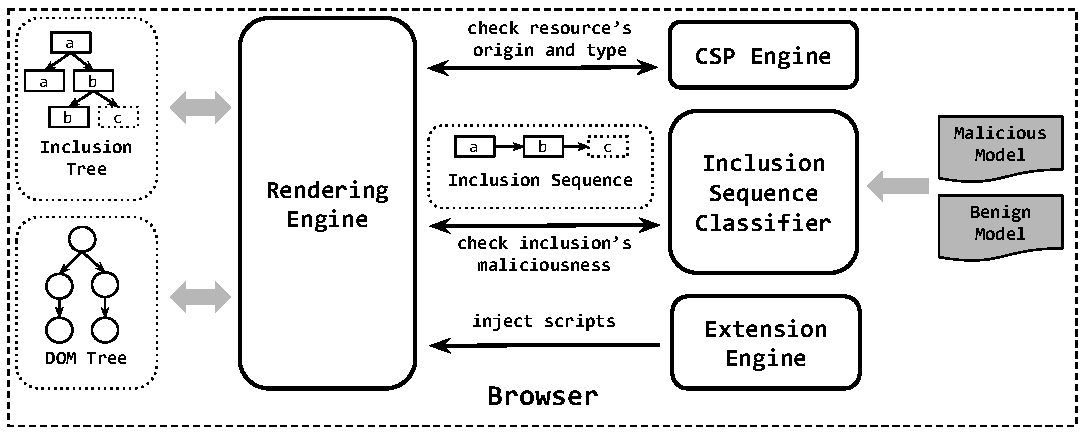
\includegraphics[width=0.9\textwidth]{inclusion/figures/inclusion_architecture}
    \caption{An overview of \excision.}
    \label{inclusion:fig:architecture}
\end{figure*}


In this section, we describe the design of \excision, our approach for detecting
and blocking the inclusion of malicious third-party content in real-time. An
overview of our system is shown in Figure~\ref{inclusion:fig:architecture}.
\excision operates by extracting resource \emph{inclusion trees} from within the
browser. The inclusion tree precisely records the inclusion relationships
between different resources in a web page. When the user requests a web page,
the browser retrieves the corresponding HTML document and passes it to the
rendering engine. The rendering engine incrementally constructs an inclusion
tree for the DOM and begins extracting external resources such as scripts and
frames as it reaches new HTML tags. For inclusion of a new resource, the
rendering engine consults the CSP engine and the \emph{inclusion sequence
classifier} in order to decide whether to include the resource. If the
resource's origin and type are whitelisted in the CSP rules, the rendering
engine includes the resource without consulting the inclusion sequence
classifier and continues parsing the rest of the HTML document. Otherwise, it
extracts the \emph{inclusion sequence} (path through the page's inclusion tree)
for the resource and forwards this to the inclusion sequence classifier. Using
pre-learned models, the classifier returns a decision about the malice of the
resource to the rendering engine. Finally, the rendering engine discards the
resource if it was identified as malicious. The same process occurs for
resources that are included dynamically during the execution of extension
content scripts after they are injected into the page.

\subsubsection{Inclusion Tree}

\begin{figure}[t]
   \centering
   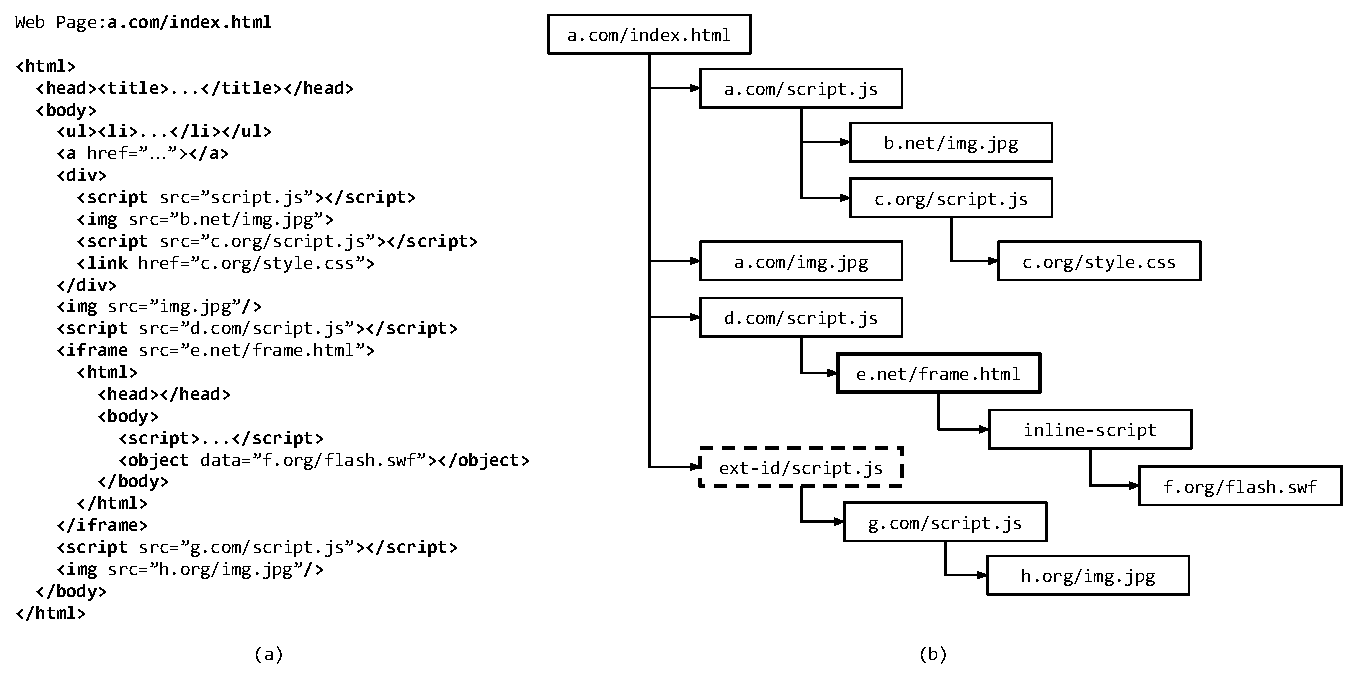
\includegraphics[width=\textwidth]{inclusion/figures/dom_inclusion_tree}
   \caption{(a) DOM Tree, and (b) Inclusion Tree}
   \label{inclusion:fig:dom_inclusion_tree}
\end{figure}


A website can include resources in an HTML document from any origin so long as
the inclusion respects the same origin policy, its standard exceptions, or any
additional policies due to the use of CSP, CORS, or other access control
framework. A first approximation to understanding the inclusions of third-party
content for a given web page is to process its DOM tree~\cite{domtree} while the
page loads. However, direct use of a web page's DOM tree is unsatisfactory
because the DOM does not in fact reliably record the inclusion relationships
between resources referenced by a page. This follows from the ability for
JavaScript to manipulate the DOM at run-time using the DOM API.

Instead, in this work we define an \emph{inclusion tree} abstraction extracted
directly from the browser's resource loading code. Unlike a DOM tree, the
inclusion tree represents how different resources are included in a web page
that is invariant with respect to run-time DOM updates. It also discards
irrelevant portions of the DOM tree that do not reference remote content.

Furthermore, browser extensions can also manipulate the web page by injecting
and executing JavaScript code in the page's context. Hence, the injected
JavaScript is considered a direct child of the root node in the inclusion tree.
An example of a DOM tree and its corresponding inclusion tree is shown in
Figure~\ref{inclusion:fig:dom_inclusion_tree}. As shown in
Figure~\ref{inclusion:fig:dom_inclusion_tree}b, \texttt{f.org/flash.swf} has
been dynamically added by an \texttt{inline script} to the DOM tree. Moreover,
\texttt{ext-id/script.js} is injected by an extension as the direct child of the
root resource. This script then included \texttt{g.com/script.js}, which in turn
included \texttt{h.org/img.jpg}.

\subsubsection{Inclusion Sequence (Chain)}

\begin{figure}
    \centering
    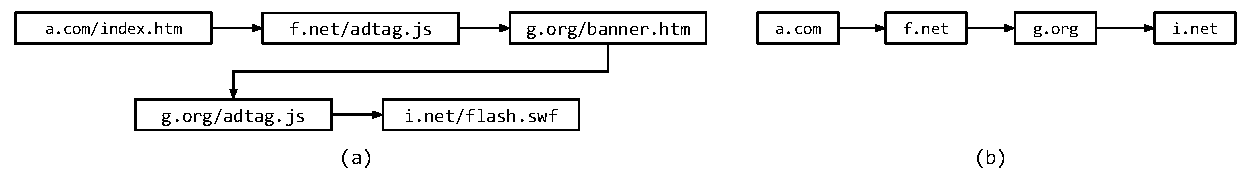
\includegraphics[width=0.9\textwidth]{inclusion/figures/inclusion_sequence}
    \caption{(a) URL Inclusion Sequence, and (b) Domain Inclusion Sequence}
    \label{inclusion:fig:inclusion_sequence}
\end{figure}


For each resource in the inclusion tree, there is an \emph{inclusion sequence
(chain)} that begins with the root resource (i.e., the URL of the web page) and
terminates with the corresponding resource. For instance, the inclusion sequence
of \texttt{f.org/flash.swf} has a length of 4 since we remove the
\texttt{inline} resources from inclusion sequence.

When we consider the full URL for constructing an inclusion sequence, the
resulting sequence is called a \emph{URL Inclusion Sequence}.
Figure~\ref{inclusion:fig:inclusion_sequence}a shows the URL inclusion sequence
of the resource \texttt{i.net/flash.swf}. However, some malware campaigns change
their URL patterns frequently to avoid detection. This can be done by changing
the URL path and the parameter values~\cite{ccs2012madtracer}. To overcome this
problem and capture the high-level relationships between different websites, we
only consider the domain part of the URL to build the \emph{Domain Inclusion
Sequence}. Figure~\ref{inclusion:fig:inclusion_sequence}b shows the domain
inclusion sequence corresponding to the aforementioned URL inclusion sequence.
As depicted, if consecutive URLs in a sequence have the same domains, we merge
them into one node. From now on, by inclusion sequence, we refer to a domain
inclusion sequence unless we mention URL inclusion sequence explicitly.

\subsubsection{Inclusion Sequence Classification}
\label{inclusion:sec:classification}

Given an inclusion sequence, \excision must classify it as benign or malicious
based on features extracted from the sequence. The task of the \emph{inclusion
sequence classifier} is to assign a class label from the set
\texttt{\{benign,malicious\}} to a given sequence based on previously learned
models from a labeled data set. In our definition, a malicious sequence is one
that starts from the root URL of a web page and terminates in a URL that
delivers malicious content. For classification, we used hidden Markov models
(HMM)~\cite{ieee1989hmm}. Models are comprised of states, each of which holds
transitions to other states based on a probability distribution. Each state can
probabilistically emit a symbol from an alphabet. There are other sequence
classification techniques such as Na\"{i}ve Bayes~\cite{ecml1998naivebayes}, but
we used an HMM for our classifier because we also want to model the
inter-dependencies between the resources that compose an inclusion sequence.

In the training phase, the system learns two HMMs from a training set of labeled
sequences, one for the benign class and one for the malicious class. We
estimated the HMM parameters by employing the Baum-Welch algorithm which finds
the maximum likelihood estimate of these parameters based on the set of observed
sequences. In our system, we empirically selected 20 for the number of states
that are fully connected to each other. In the subsequent detection phase, we
compute the likelihood of a new sequence given the trained models using the
forward-backward algorithm and assign the sequence to the class with the highest
likelihood. Training hidden Markov models is computationally expensive. However,
computing the likelihood of a sequence is instead very efficient, which makes it
a suitable method for real-time classification~\cite{ieee1989hmm}.

\subsubsection{Classification Features}
\label{inclusion:sec:features}

Let $r_0 \rightarrow r_1 \rightarrow \dots \rightarrow r_n$ be an inclusion
sequence as described above. Feature extraction begins by converting the
inclusion sequence into sequences of feature vectors. After analyzing the
inclusion trees of several thousands benign and malicious websites for a period
of 11 months, we identified 12 feature types from three categories. For each
feature type, we compute two different features: individual and relative
features. An individual feature value is only dependent on the current resource,
but a relative feature value is dependent on the current resource and its
preceding (or parent) resources. Consequently, we have 24 features for each
resource in an inclusion sequence. Individual features can have categorical or
continuous values. All continuous feature values are normalized on
$\left[0,1\right]$ and their values are discretized. In the case of continuous
individual features, the relative feature values are computed by comparing the
individual value of the resource to its parent's individual value. The result of
the comparison is \texttt{less}, \texttt{equal}, or \texttt{more}. We use the
value \texttt{none} for the root resource. To capture the high-level
relationships between different inclusions, we only consider the domain part of
the URL for feature calculation.

\paragraph{DNS-based Features}

The first feature category that we consider is based on DNS properties of the
resource's domain.

\begin{table}[t]
    \centering
    \footnotesize
    \label{inclusion:tab:tld}
    \caption{TLD values}
    \begin{subtable}{.43\textwidth}
        \centering
        \caption{Individual}
        \label{inclusion:tab:tld:individual}
        \begin{tabular}{ll}
        \toprule
        \textbf{Value} & \textbf{Example} \\
        \midrule
        \texttt{none} & IPs, Extensions \\
        \texttt{gen} & *.com, *.org \\
        \texttt{gen-subdomain} & *.us.com \\
        \texttt{cc} & *.us, *.de, *.cn \\
        \texttt{cc-subdomain} & *.co.uk, *.com.cn \\
        \texttt{cc-int} & *.xn{-{}-}p1ai (ru) \\
        \texttt{other} & *.biz, *.info \\
        \bottomrule
        \end{tabular}
    \end{subtable}
    \begin{subtable}{.54\textwidth}
        \centering
        \caption{Relative}
        \label{inclusion:tab:tld:relative}
        \begin{tabular}{ll}
        \toprule
        \textbf{Value} & \textbf{Example} \\
        \midrule
        \texttt{none} & root resource \\
        \texttt{\{got,lost\}-tld} & Ext. $\rightarrow$ *.de, *.us $\rightarrow$ IP \\
        \texttt{gen-to-\{cc,other\}} & *.org $\rightarrow$ \{*.de, *.info\} \\
        \texttt{cc-to-\{gen,other\}} & *.uk $\rightarrow$ \{*.com, *.biz\} \\
        \texttt{other-to-\{gen,cc\}} & *.info $\rightarrow$ \{*.net, *.uk\} \\
        \texttt{same-\{gen,cc,other\}} & *.com $\rightarrow$ *.com \\
        \texttt{diff-\{gen,cc,other\}} & *.info $\rightarrow$ *.biz \\
        \bottomrule
        \end{tabular}
    \end{subtable} 
\end{table}


\begin{table}[t]
    \centering
    \footnotesize
    \label{inclusion:tab:type}
    \caption{Type values}
    \begin{subtable}{.43\textwidth}
        \centering
        \caption{Individual}
        \label{inclusion:tab:type:individual}
        \begin{tabular}{ll}
            \toprule
            \textbf{Value} & \textbf{Example} \\
            \midrule
            \texttt{ipv6} & 2607:f0d0::::4 \\
            \texttt{ipv4-private} & 192.168.0.1 \\
            \texttt{ipv4-public} & 4.2.2.4 \\
            \texttt{extension} & Ext. Scripts \\
            \texttt{dns-sld} & google.com \\
            \texttt{dns-sld-sub} & www.google.com \\
            \texttt{dns-non-sld} & abc.dyndns.org \\
            \texttt{dns-non-sld-sub} & a.b.dyndns.org \\
            \bottomrule
        \end{tabular}
    \end{subtable}
    \begin{subtable}{.54\textwidth}
        \centering
        \caption{Relative}
        \label{inclusion:tab:type:relative}
        \begin{tabular}{ll}
            \toprule
            \textbf{Value} & \textbf{Example} \\
            \midrule
            \texttt{none} & root resource \\
            \texttt{same-site} & w.google.com $\rightarrow$ ad.google.com \\
            \texttt{same-sld} & 1.dyndns.org $\rightarrow$ 2.dyndns.org \\
            \texttt{same-company} & ad.google.com $\rightarrow$ www.google.de \\
            \texttt{same-eff-tld} & bbc.co.uk $\rightarrow$ london.co.uk \\
            \texttt{same-tld} & bbc.co.uk $\rightarrow$ london.uk \\
            \texttt{different} & google.com $\rightarrow$ facebook.net \\
            \bottomrule
            \\
        \end{tabular}
    \end{subtable} 
\end{table}


\begin{itemize}

\item \textbf{Top-Level Domain}: For this feature, we measure the types of TLDs
from which a resource is included and how it changes along the inclusion
sequence. For every resource in an inclusion sequence, we assign one of the
values in Table~\ref{inclusion:tab:tld:individual} as an individual feature. For
the relative feature, we consider the changes that occur between the top-level
domain of the preceding resource and the resource itself.
Table~\ref{inclusion:tab:tld:relative} shows 15 different values of the relative
TLD feature.

\item \textbf{Type}: This feature identifies the types of resource domains and
their changes along the inclusion sequence. Possible values of individual and
relative features are shown in Table~\ref{inclusion:tab:type:individual} and
Table~\ref{inclusion:tab:type:relative} respectively.

\item \textbf{Level}: A domain name consists of a set of labels separated by
dots. We say a domain name with $n$ labels is in level $n-1$. For example,
\texttt{www.google.com} is in level 2. For IP addresses and extension scripts,
we consider their level to be 1. For a given domain, we compute the individual
feature by dividing the level by a maximum value of 126.

\item \textbf{Alexa Ranking}: We also consider the ranking of a resource's
domain in the Alexa Top 1M websites. To compute the normalized ranking as an
individual feature, we divide the ranking of the domain by one million. For IP
addresses, extensions, and domains that are not in the top 1M, we use the value
\texttt{none}.

\end{itemize}

\paragraph{String-based Features}

In this feature category, we characterize the string properties of resource
domains. For IP addresses and extension scripts, we assign the value 1 for
individual features.

\begin{itemize}

\item \textbf{Non-Alphabetic Characters}: For this feature, we compute the
individual feature value by dividing the number of non-alphabetical characters
over the length of domain.

\item \textbf{Unique Characters}: We also measure the number of unique
characters that are used in a domain. The individual feature is the number of
unique characters in the domain divided by the maximum number of unique
characters in the domain name, which is 38 (26 alphabetics, 10 digits, hyphen,
and dot).

\item \textbf{Character Frequency}: For this feature, we simply measure how
often a single character is seen in a domain. To compute an individual feature
value, we calculate the frequency of each character in the domain and then
divide the average of these frequencies by the length of the domain to normalize
the value.

\item \textbf{Length}: In this feature, we measure the length of the domain
divided by the maximum length of a domain, which is 253.

\item \textbf{Entropy}: We employ Shannon entropy to measure the randomness of
domains in the inclusion sequence. We calculate normalized entropy as the
absolute Shannon entropy divided by the maximum entropy for the domain name.

\end{itemize}

\paragraph{Role-based Features}

We consider three roles for a resource:
\begin{inparaenum}[\itshape i)\upshape]
     \item ad-network,
     \item content delivery network (CDN), and
     \item URL shortening service.
\end{inparaenum}
In total, we have three features in this category, as each domain can
simultaneously perform multiple roles. Both individual and relative features in
this category have binary values.
